\documentclass{sigchi}

% Use this command to override the default ACM copyright statement (e.g. for preprints).
% Consult the conference website for the camera-ready copyright statement.


%% EXAMPLE BEGIN -- HOW TO OVERRIDE THE DEFAULT COPYRIGHT STRIP -- (July 22, 2013 - Paul Baumann)
% \toappear{Permission to make digital or hard copies of all or part of this work for personal or classroom use is 	granted without fee provided that copies are not made or distributed for profit or commercial advantage and that copies bear this notice and the full citation on the first page. Copyrights for components of this work owned by others than ACM must be honored. Abstracting with credit is permitted. To copy otherwise, or republish, to post on servers or to redistribute to lists, requires prior specific permission and/or a fee. Request permissions from permissions@acm.org. \\
% {\emph{CHI'14}}, April 26--May 1, 2014, Toronto, Canada. \\
% Copyright \copyright~2014 ACM ISBN/14/04...\$15.00. \\
% DOI string from ACM form confirmation}
%% EXAMPLE END -- HOW TO OVERRIDE THE DEFAULT COPYRIGHT STRIP -- (July 22, 2013 - Paul Baumann)


% Arabic page numbers for submission.
% Remove this line to eliminate page numbers for the camera ready copy
% \pagenumbering{arabic}


% Load basic packages
\usepackage{balance}  % to better equalize the last page
\usepackage{graphics} % for EPS, load graphicx instead
\usepackage{times}    % comment if you want LaTeX's default font
\usepackage{url}      % llt: nicely formatted URLs

% llt: Define a global style for URLs, rather that the default one
\makeatletter
\def\url@leostyle{%
  \@ifundefined{selectfont}{\def\UrlFont{\sf}}{\def\UrlFont{\small\bf\ttfamily}}}
\makeatother
\urlstyle{leo}


% To make various LaTeX processors do the right thing with page size.
\def\pprw{8.5in}
\def\pprh{11in}
\special{papersize=\pprw,\pprh}
\setlength{\paperwidth}{\pprw}
\setlength{\paperheight}{\pprh}
\setlength{\pdfpagewidth}{\pprw}
\setlength{\pdfpageheight}{\pprh}

% Make sure hyperref comes last of your loaded packages,
% to give it a fighting chance of not being over-written,
% since its job is to redefine many LaTeX commands.
\usepackage[pdftex]{hyperref}
\hypersetup{
pdftitle={SIGCHI Conference Proceedings Format},
pdfauthor={LaTeX},
pdfkeywords={SIGCHI, proceedings, archival format},
bookmarksnumbered,
pdfstartview={FitH},
colorlinks,
citecolor=black,
filecolor=black,
linkcolor=black,
urlcolor=black,
breaklinks=true,
}

% create a shortcut to typeset table headings
\newcommand\tabhead[1]{\small\textbf{#1}}


% End of preamble. Here it comes the document.
\begin{document}

\title{JobFinder: A Personalized Resume-Job Matching System}

\numberofauthors{3}
\author{
  \alignauthor 1st Author Name\\
    \affaddr{Affiliation}\\
    \affaddr{Address}\\
    \email{e-mail address}\\
    \affaddr{Optional phone number}
  \alignauthor 2nd Author Name\\
    \affaddr{Affiliation}\\
    \affaddr{Address}\\
    \email{e-mail address}\\
    \affaddr{Optional phone number}
  \alignauthor 3rd Author Name\\
    \affaddr{Affiliation}\\
    \affaddr{Address}\\
    \email{e-mail address}\\
    \affaddr{Optional phone number}
}

\maketitle

\begin{abstract}
Today, online recruiting web sites such as Monster and Indeed have become one of the main channels for people to find jobs. These web platforms have provided their services for more than ten years, and have saved a lot of time and cost for both job seekers and organizations who want to hire people. However, traditional information retrieval techniques may not be appropriate for users. The reason is because the number of results returned to a job seeker may be huge, so job seekers are required to spend a significant amount of time reading and reviewing their options. One popular approach to resolve this difficulty for users are recommender systems, which is a technology that has been studied for a long time. This proposal will present a personalized resume-job matching system, which will obtain the models from the job descriptions and resumes, and use ontology techniques to find appropriate jobs for job seekers.
\end{abstract}

\keywords{
	Guides; instructions; author's kit; conference publications;
	keywords should be separated by a semi-colon. \newline
	\textcolor{red}{Optional section to be included in your final version,
  but strongly encouraged.}
}

\category{H.5.m.}{Information Interfaces and Presentation (e.g. HCI)}{Miscellaneous}

See: \url{http://www.acm.org/about/class/1998/}
for more information and the full list of ACM classifiers
and descriptors. \newline
\textcolor{red}{Optional section to be included in your final version,
but strongly encouraged. On the submission page only the classifiers��
letter-number combination will need to be entered.}


\section{Introduction}

Currently the main channel for job seekers are online job finding web sites, like indeed or  monster etc, that make the job finding process easier and decrease the recruitment time. But most such web sites only allow users to use key word to search the jobs, which makes job searching as tedious and blind task. For example, I used keyword ``Java'' to search jobs with location restriction Mountain View, CA on the job searching site indeed.com, the web site returned about 7,000 jobs (Figure~\ref{fig:Indeed}). The number of results of job searching is huge but un-ranked, so the job seeker has to review every job description. Since no one has enough time to read all the jobs in the searching result, the actual quality of job searching service is low. This is a classic problem of information overflow.


\begin{figure}[htbp]
  \centering
  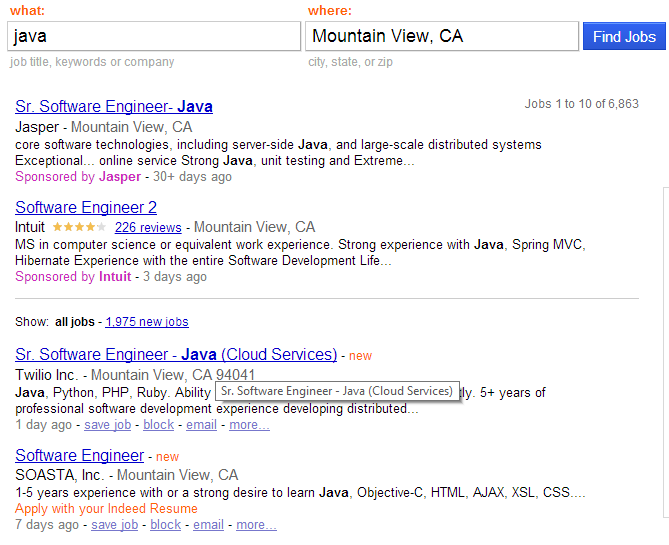
\includegraphics[scale=0.4]{images/indeed1.png}
  \caption{Search result of Indeed}
  \label{fig:Indeed}
\end{figure}

The reason for such result is because current job searching web sites use the same information retrieval technology like ``Inverted index'' \cite{zobel2006inverted} as the common search engines, which just use keywords to map all the stored documents. Modern search engines all have some ranking algorithms to sort the searching result, like page rank \cite{page1999pagerank}, so the top results always be the most related ones. But such algorithms are unavailable to the job searching systems, because the criteria  of how to rank the job searching result is very personalized. A great job opening for one job seeker maybe looks not good to the other, because the goodness of a job to a specular job seeker is heavily depend on his personal background, like his education or professional experience etc.

Since the people's resumes contain the most important background information, we believe the content of the resume could be used to rank the job openings. My proposal is to create a web system which could use the resumes of job seekers to find the jobs that match their profiles best. The main idea is to calculate the similarity between the candidate model and job models, which should be generated from resumes and job descriptions. I want to transfer the job searching task from key word searching to candidate model matching. The matching result should be sorted by the matching score, higher matching score means a better matching. The matching algorithm not only help job seekers to find the appreciate job opening, but also offer priority to them.~\cite{gueutal2006brave}  The job with higher matching score means the job is more appropriate to the job seeker, and if he applies the job, the chance of getting the interview will be higher as well. Figure~\ref{fig:Matching} shows how this approach works.


\begin{figure}[htbp]
  \centering
  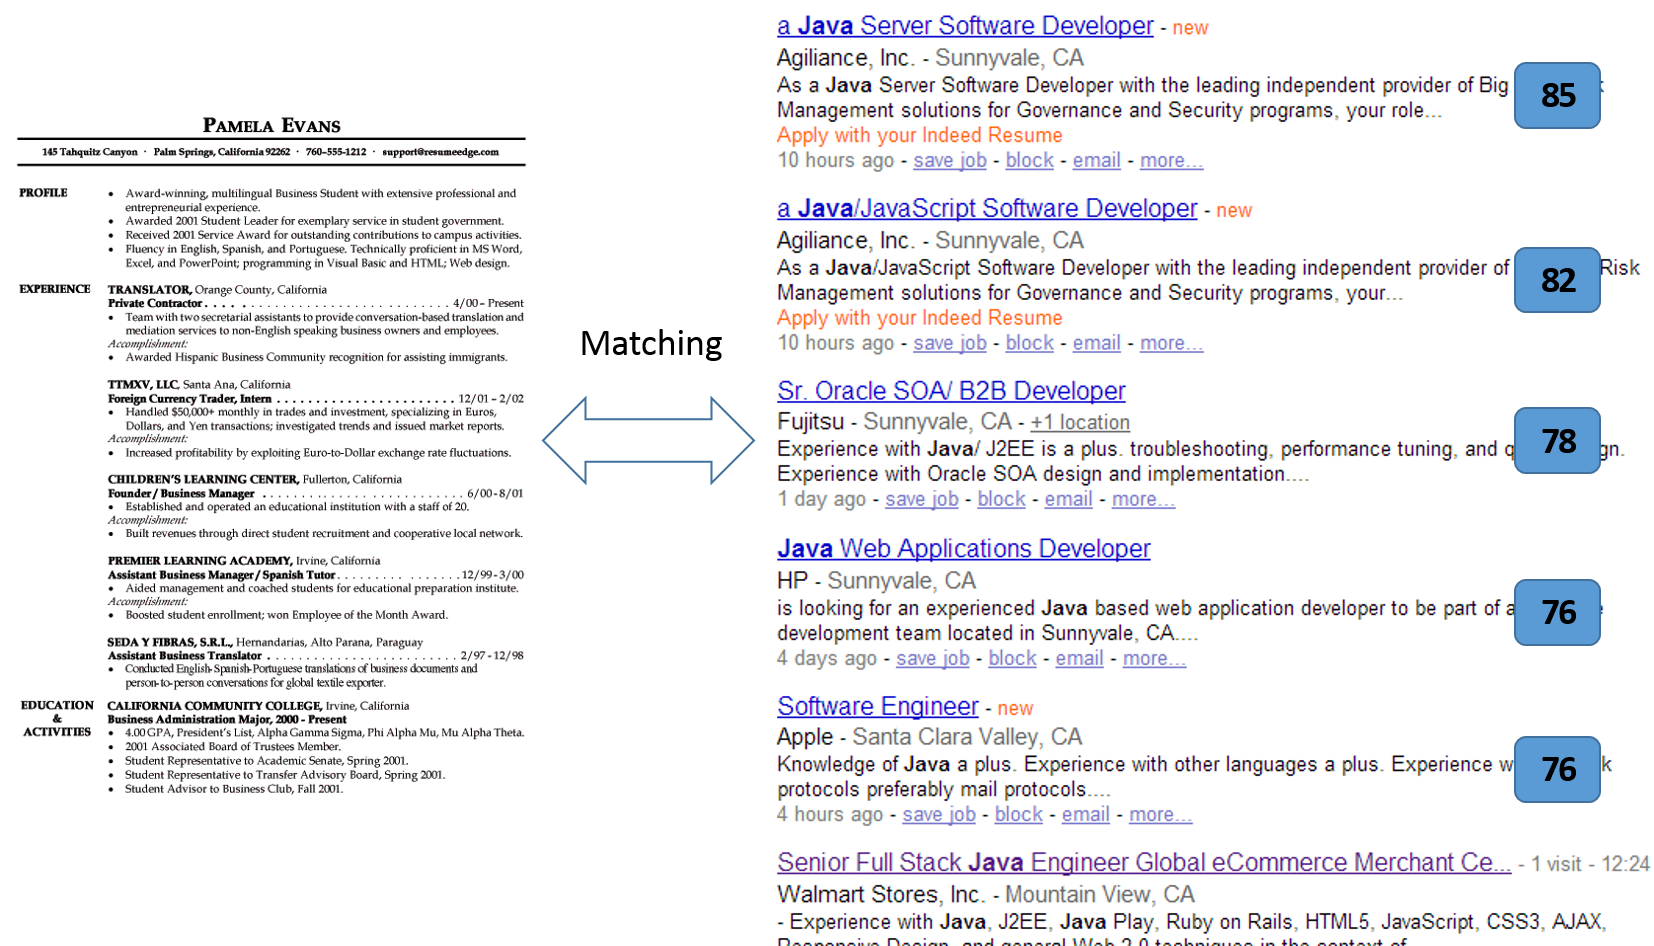
\includegraphics[scale=0.5]{images/matching.png}
  \caption{Matching the job opening with Resume}
  \label{fig:Matching}
\end{figure}

\subsection{Contribution}

we make the following contributions in this work:

\begin{enumerate}
    \item  We create a finite automata based matching tool to extract information from text.
    \item  We define some pattern for labeled text to extract information.
    \item  We create a domain specific Ontology for recruitment.
    \item  We proposed statistical based Ontology similarity measure.
    \item  We proposed a approach to calculate the similarity between job and resume.
\end{enumerate}

\subsection{Organizations}
The subsequent chapters are organized as follows: We first describe what has been done in terms of prior work.  We introduce some basic conception of recommender systems, and how to apply recommendation approached into Job Recommender Systems. Some previous Job Recommender Systems will be introduced and their advantages and limits will be discussed. Then two import problems of content-based Job Recommender Recommender Systems, Information Extraction and Similarity Calculation, will be

We then propose a finite automata matching tool which match pattern in sentence, and extract related information. We will compare this tool to some others tools, demonstrate its flexibility. Some patterns will be presented.

Ontology play an important role in this system. We will present how to construct the domain specific Ontology. We also give a brief review of different Ontology similarity measures. We proposed a statistical-based Ontology Similarity measure. The algorithm will be presented, and some evaluation will be given.

Finally, we evaluate our system by using some pre-collected data from Internet. Using our improved algorithm we were able to achieve an accuracy of 90\% for a 10 digit gesture set, 82\% accuracy for the 26 English characters and over 95\% accuracy for a set of seven commonly used gestures.

\section{Related Works}


Rafter et al. \cite{rafter2000personalised} began to use ACF (Automated Collaborative Filtering) in Job Recommender system, ``CASPER''. In the system user profiles are gotten from server logs, that included: revisit data, read time data, and activity data. All these factors were viewed as measure of relevance among users. The system recommend jobs in two steps. First the system find a set of user related to the target user, second the jobs that related users liked will be recommend to the target user. The system use cluster-based Collaborative Filtering strategy. The similarity between users are based on how many jobs they both reviewed, or applied.

The CASPER also allows user search jobs by a query which is a combination of some fields, like location, salary, and skill etc. The system use such query to find jobs, and the returned jobs will be ranked with above collaborative filtering algorithm.
In their paper, they didn't give a detail description on how to detect the related fields they need and how to the transfer semi-structured job description to structured one. This system is helping job seeker to find jobs.

The shortage of Collaborative Filtering:
 First since the searching result is huge, and the result is sorted randomly, even two very similar users may review different jobs,  or say the probability of two similar users reviewing the same job is low. The authors also noticed the such sparseness problem in users profile, so they try to user cluster-based solution to resolve this problem.

 Second because recommended jobs are from others users searching result, since the current quality of current searching result is low, so the quality of recommendation cannot be high.

F{\"a}rber et al \cite{farber2003automated}. presented a recommender system built on a hybrid approach. The system integrated two methods, content-based filtering and collaborative filtering, and tried to overcome the problem of rating data sparsity by leveraging synergies of a combined model, et. the  latent aspect model. The data they used were synthetic resume. The model they are shown in Figure


\begin{figure}[htbp]
  \centering
  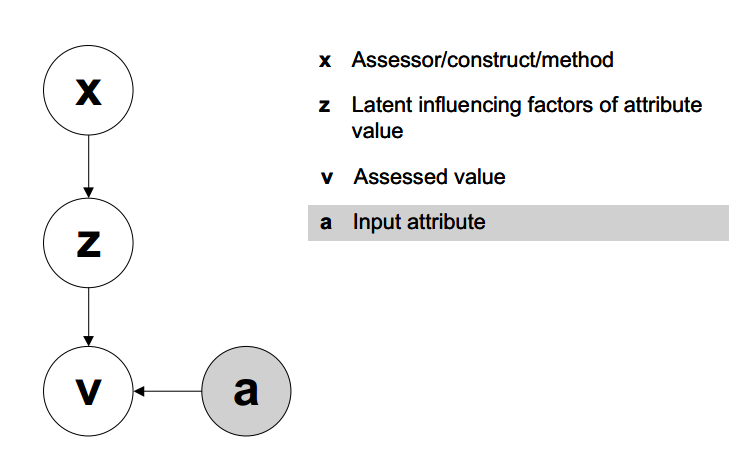
\includegraphics[scale=0.4]{images/la.png}
  \caption{Latent Aspect Model}
  \label{fig:la}
\end{figure}

In Malinowski et al. \cite{malinowski2006matching}, they classified the job recommender systems into two categories,  CV-recommender, which to recommend CVs to recruiter. The job-recommender, which recommend jobs to job seekers.

The system collect the users' profile data by asking input their profiles to the web form based interface field by field. The input data collected are:

\begin{enumerate}
    \item  Demographic data (e.g. date of birth, contact information)

    \item  Educational data (e.g. school courses, grades, university, type of degree, intermediate and final university examinations, postgraduate studies)

    \item  Job experience (e.g. name of the company, type of employment, industry group, occupational field)
    \item  Language skills (e.g. language, level of knowledge)
    \item  IT skills (e.g. type of skill, level of knowledge)
    \item  Awards, scholarships, publications, others

\end{enumerate}


The system also asked the users upload their resumes, but that's for facilitating the human judgment.

From the paper we know, the model latent aspect model is statistical model, which need to be trained before be applied into recommendation. But training need user to label to data, since current quality of result of job searching is poor, it will take a lot of time for user to train model.


Drigas* et al.\cite{malinowski2006matching} al presented a expert system to match jobs and job seekers, and recommend unemployed to  The expert system used Neuro-Fuzzy rule to evaluate the matching:
Candidate's X matches X Criterion




The system represent the job in six fields:
\begin{enumerate}
    \item  Age
    \item  Education
    \item  Additional Education(Training)
    \item  Previous Employment (Experience)
    \item  Foreign Language
    \item  Computer Knowledge
\end{enumerate}


 The system use a relation matrix to represent the fuzzy relation between these specialities. The system need the training data to train that Neuro-fuzzy network.

Both resume data and job info data were manually input into the system  . The fields they selected are relative small.

Daramola et al.  also proposed a fuzzy logic based expert system(FES) tool for online personnel resctuitments. In the paper, the authors assumed that the information already be collected. The system use a fuzzy distance metric to rank candidates' profile in the order of their eligibility for the job. The fuzy hamming distance is given as:
$$ \delta \left ( O,R \right )=\sum_{i=1}^{n}\left | \mu_O(x_i) - \mu_R(x_i)  \right | $$

Ioannis et al. used a machine learned prediction model to recommend new jobs to job seekers~\cite{paparrizos2011machine}.  The features used by the prediction model includes:



\begin{table}[ht]
\caption{Resume and Job Description} % title of Table
\centering % used for centering table
\begin{tabular}{ l l r }
 \hline
 Feature type &  Feature  &  Range   \\ \hline
              &  company title   & String  \\
Institution   &  industry        & String  \\
              &  company type    & \{public, private\} \\
              &  number of employees &    Num \\
 \hline
              &  number of jobs         & Num  \\
              &  position title         & String  \\
  employee    &  best position title    & String \\
              &  years of experience    &    Num \\
              &  number of universities &    Num \\
              &  education degree       & String \\
 \hline
\end{tabular}
\label{tab:predictionmodel} % is used to refer this table in the text
\end{table}



when applying a job, the common method is let the candidates upload their resumes, sometimes the company want user to enter details like personal information, education and experience details, skills. However, in real life, the candidates do not input a lot information in the on-line form. ~\cite{singh2010prospect}

Some big IT companies had meet a similar problem of information overflow. Any position they published, will receive a lot applications, the recruiter need to screen the all the applications, but this task is also tedious and time consuming, highly cumbersome and inefficient. so these company tried to build the system to help screen the position candidates.

Amit et al. in IBM presented a system, ``PROSPECT'', ~\cite{singh2010prospect} to aid in the shortlisting of candidates for jobs. The system uses a resume miner to extract the information from resumes, which use a CRF model to segment and label the resumes. The CRF model used three kinds of features, they are: Lexicon, Visual, Named Entity, Text, and Conjunction. The paper compared some algorithms to ranked the candidates applicants, such methods include: Okapi BM25, KL, Lucene Scoring, and Lucene Scoring + SkillBoost.

HP also built a system to solve the similar problem, which was introduced in Gonzalez et al.'s paper ~\cite{gonzalez2012adaptive}. The system also pay a lot of attention to information extraction. The IE architecture they use is shown in figure ~\ref{fig:hpie}.


\begin{figure}[htbp]
  \centering
  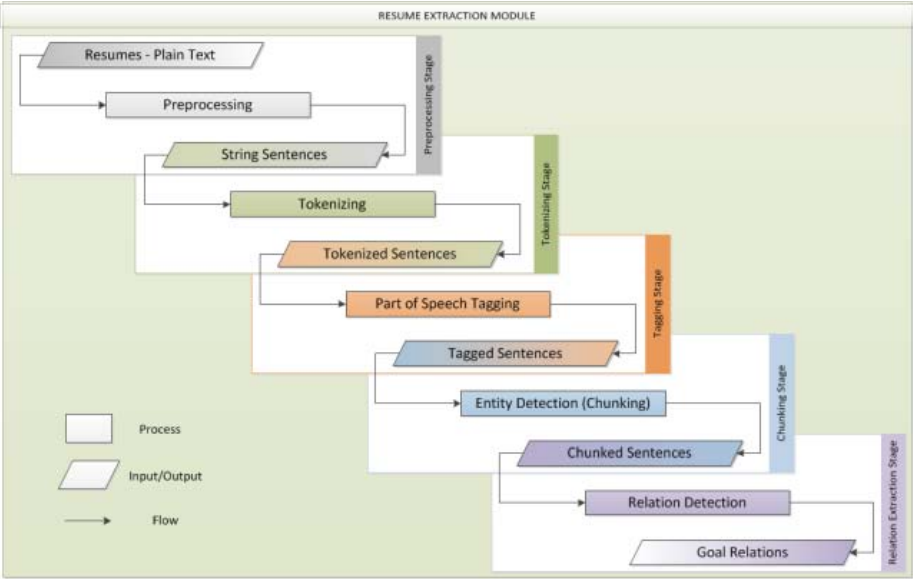
\includegraphics[scale=0.5]{images/hpie.png}
  \caption{IE Framework}
  \label{fig:hpie}
\end{figure}

The scholars in this paper, the dictionaries which were used to tag entities should be updated often since there always new terms appears. So an adaptive learning module was used to achieve two objectives: use semantic data to enhance the information extraction and to discover new terms.
A domain-oriented ontology is used to represent knowledge, inference rules are defined based on the ontology knowledge base. When a detected term found, the system will search in external knowledge base, like DBpedia etc. The resume also be classified to different categories like ``Web Technology'' and ``No Web Technology'' by naive Bayes classifier. The company could allocate appropriate employees to required positions.


Yao et al.~\cite{lu2013recommender} also presented a hybrid recommender system which integrated content-based and interaction-based relation. In content-based part, relations between job-job, job-job seeker, and job seeker - job seeker could be identified by their similarity of profiles.

There two approaches are used to calculate the similarities: For the structured data, like age gender  etc., the weight sum values will be returned, for the unstructured data like similarity between job and user profile the Latent Semantic Analysis will be used.

This system was build on the assumption: The users with similar profiles tend to have similar interests. But here we could find two problems: At first, people with similar profile may not have similar interest, this is a very common fact. For example two students both graduate from same department with the same degree at the same year, when they look for jobs, they may have different preference. Second, to job's part, the accuracy of similarity calculation will effect a lot on the result of the system, since two very similar job may be classified as different jobs in the system.





Yu et al.~\cite{yu2005resume} used a cascaded information extraction (IE) framework to get the detailed information from the job seeker��s resume. In the first stage, the Hidden Markov Modeling (HMM) model is used to segment the resume into consecutive blocks. Based on the result, a SVM model is used to obtain the detailed information in the certain block, the information include: name, address, education etc.

 Celik Duygua and Elci Atilla proposed a Ontology-based R��sum�� Parser (ORP) ~\cite{ccelik2013ontology}, which uses ontology to assistant the information extraction process. The system process the resume in following steps: convert the resume files into plain text, separate the text into  some segments, use Ontology Knowledge Base to find the concepts in the sentences, normalize all the terms, at last the system will classify the sentences to get the wanted terms.

\section{Matching Algorithms}

Lu et al~\cite{lu2013recommender}. used latent Semantic Analysis(LSA) to calculate similarities between jobs and candidates, but they only selected two factors ``interest'' and ``education''  to compare candidates. Xing et al. ~\cite{yi2007matching} used Structured Relevance Models (SRM) to  match resumes and jobs.



\bibliographystyle{acm-sigchi}
\bibliography{jobaly}
\end{document}
